\documentclass[12pt]{article}

% ---------------------------------------------------------------------------
% Detection Without Identification -- methods-memo version (~8 pp.)
% Austin Belman and Kameron Nelson. Single-spaced working-paper version of the full paper.
% Compile: pdflatex methods_memo.tex  (run twice for cross-references)
% ---------------------------------------------------------------------------

\usepackage[T1]{fontenc}
\usepackage[utf8]{inputenc}
\usepackage[margin=1in]{geometry}
\usepackage{mathptmx}
\usepackage{graphicx}
\graphicspath{{../plots/}}
\usepackage{booktabs}
\usepackage{amsmath}
\usepackage{array}
\usepackage{float}
\usepackage{caption}
\captionsetup{font=small,labelfont=bf,justification=raggedright,singlelinecheck=false}
\usepackage[hidelinks]{hyperref}

\setlength{\parindent}{0.4in}
\renewcommand{\arraystretch}{1.2}

\title{\vspace{-1.5em}\textbf{Detection Without Identification: A Validity Assessment of the
ShotSpotter Difference-in-Differences Design in Chicago, 2009--2023}}
\author{Austin Belman and Kameron Nelson}
\date{June 2026}

\begin{document}

\maketitle
\thispagestyle{empty}

\begin{abstract}
\noindent
A two-way fixed-effects difference-in-differences regression of Chicago gun homicides on
ShotSpotter installation returns a positive, statistically significant estimate of
$+2.63$ homicides per community-area-year ($p < 0.001$). We show that the estimate is an
artifact of two choices rather than a treatment effect. Modeling integer homicide counts
with ordinary least squares inflates the coefficient; estimated by Poisson or Negative
Binomial regression with the same fixed effects, the effect falls to an incidence-rate
ratio of $1.07$ (95\% CI $[0.87, 1.33]$, $p = 0.51$), a statistically null result. The
design also fails the conditions difference-in-differences requires. A joint Wald test
rejects parallel pre-trends ($F = 19.9$, $p = 0.006$). Treatment dates assigned to
pre-rollout years (1999, 2003) produce coefficients of comparable magnitude and
significance to the post-2017 estimate. Synthetic control is infeasible because the 26
never-treated community areas are lower-violence than any treated neighborhood, so no
donor pool reproduces a treated unit. The Callaway and Sant'Anna (2021) estimator returns
a negative overall effect that reverses sign when a single outlier year (2016) is
dropped. Across every design the data do not identify a causal effect of ShotSpotter on
gun homicides in either direction, and they are inconsistent with a large deterrence
effect of the kind a \$3 million detection contract was expected to produce. The methodological lesson
generalizes: a coefficient can survive fixed effects and robustness restrictions and
still reflect specification choice and a design without a valid counterfactual.
\end{abstract}

\section{Introduction}

Acoustic gunshot detection promises to close a measurement gap. About one in five
shootings is reported to police (Irvin-Erickson et al., 2016), so a sensor network that
flags gunfire directly could speed response and, in principle, reduce deaths. Chicago
acted on that premise. The city expanded ShotSpotter to 51 of its 77 community areas in
2017 and 2018 under a three-year, \$3 million contract, then cancelled it in 2023 after an
audit found that alerts rarely produced investigative evidence (Office of Inspector
General, 2021).

The policy question is whether the program reduced gun violence---and for Chicago it is
largely settled: district-level (Connealy et al., 2024) and national (Doucette et al.,
2021) evaluations find no crime-reduction effect, so the contribution here is the
identification assessment, not the null. The methodological question, which we treat as
primary, is whether the available data can answer the policy question at all. We estimate
the effect of ShotSpotter installation on gun homicides using a community-area-by-year
panel for 2009 to 2023, and we hold each estimate against the assumptions its design
requires. The headline difference-in-differences estimate is
positive and significant. It does not survive correct modeling of the outcome, a test of
parallel pre-trends, a placebo on pre-rollout years, or a check on the adequacy of the
comparison group. The contribution is the demonstration itself: a worked case in which a
coefficient that passes the usual robustness restrictions still fails the conditions for a
causal interpretation.

\section{Setting and data}

ShotSpotter triangulates the sound of gunfire through fixed microphones, filters
non-gunshot sounds, and forwards reviewed alerts to police (Choi, Librett, \& Collins,
2014). Chicago concentrated coverage in its highest-violence neighborhoods. From 2009 to
2016, the 51 areas that later received ShotSpotter averaged 381 gun homicides per year;
the 26 areas that never received it averaged 42, a ratio close to nine to one. Treatment
was assigned where violence was already highest. That assignment rule is the source of
every identification problem below.

The analysis combines four City of Chicago open-data products: the Violence Reduction
victims file (61,450 incidents, 1991 to 2025), filtered to gun homicides (about 7,600 in
2009 to 2023); the historical ShotSpotter alert file (222,108 alerts, January 2017 to
December 2023); the 2008 to 2012 Census socioeconomic indicators; and the community-area
boundaries. The alert file shows a staggered rollout: 21 community areas activate in 2017
and 30 in 2018, which leaves 26 never-treated areas. Pooling both cohorts at a single 2017
cutoff, the convention in the original pipeline, biases the estimate when treatment timing
varies (Goodman-Bacon, 2021); the cohort-aware estimators below address that bias.

\begin{figure}[H]
\centering
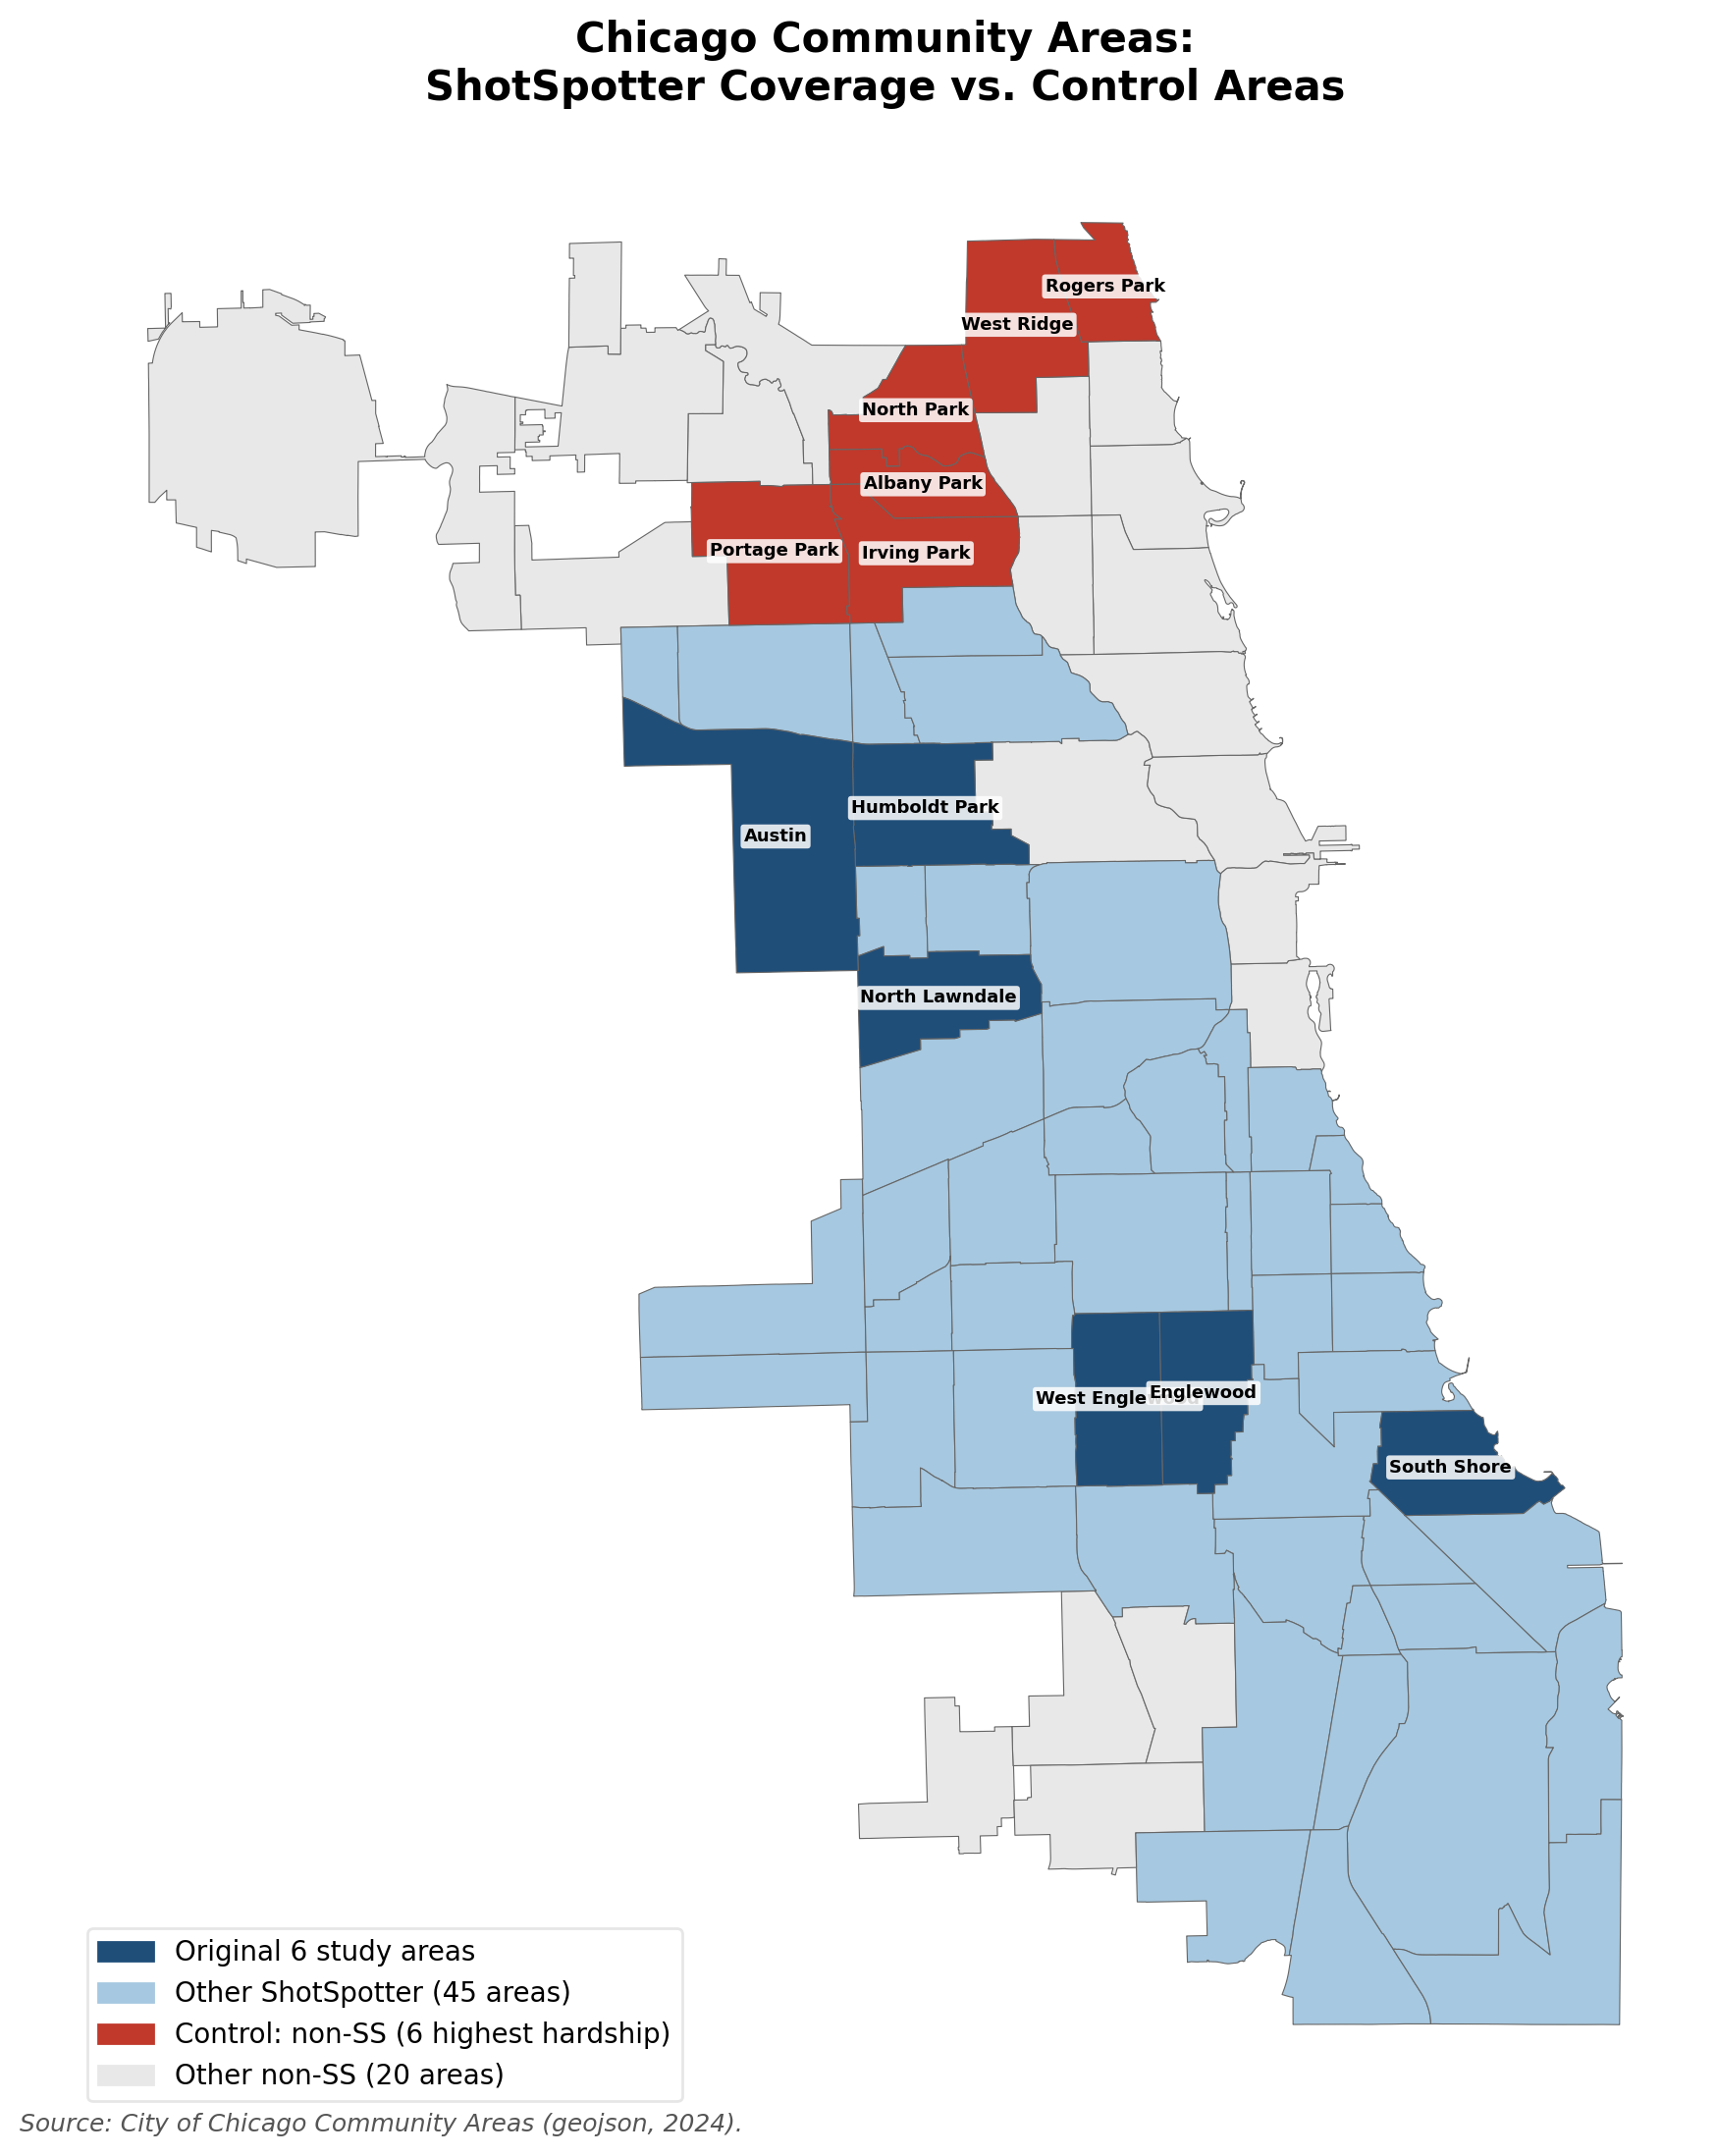
\includegraphics[width=0.66\textwidth]{did_map_treatment_control.png}
\caption{ShotSpotter coverage (blue) concentrates in the high-violence South and West
sides. The 26 never-treated community areas form the comparison group, with the six
highest-hardship areas shown in red. Treatment was assigned where violence was already
highest.}
\label{fig:map}
\end{figure}

\section{Identification and threats to inference}

Difference-in-differences identifies a causal effect only if treated and control units
would have followed parallel paths absent treatment. Chicago's data strain that condition
from the start. The treated areas began the period with roughly nine times the control
areas' homicide rate, so the comparison rests on parallel trends rather than on
comparable levels. We test the conditions the design needs and report each test against the
threat it addresses (Table~\ref{tab:threats}).

\begin{table}[H]
\centering
\small
\caption{Conditions the difference-in-differences design requires, the diagnostic for
each, and the result.}
\label{tab:threats}
\begin{tabular}{p{0.24\textwidth}p{0.26\textwidth}p{0.30\textwidth}p{0.13\textwidth}}
\toprule
Condition required & Diagnostic & Finding & Status \\
\midrule
Parallel pre-trends & Cohort event study; joint Wald $F$-test & $F = 19.9$, $p = 0.006$; pre-period effects large and negative & Rejected \\
Correct outcome model & Poisson and Negative Binomial against OLS & OLS $+2.63$ falls to IRR $1.07$ ($p = 0.51$) & OLS misspecified \\
No spurious significance & Placebo treatment in pre-rollout years & 1999 and 2003 significant at the 1\% level & Design fails \\
Adequate comparison group & Synthetic control feasibility; permutation & Single-donor solution; pre-RMSE 10--34 against levels 15--70 & Infeasible \\
Stability to staggered timing & Callaway--Sant'Anna against two-way FE & Overall effect reverses sign when 2016 is dropped & Not identified \\
\bottomrule
\end{tabular}
\end{table}

\section{Results}

\subsection{The headline estimate is a count-data artifact}

The two-way fixed-effects regression of annual gun homicides on the treatment-by-post
interaction, with community-area and year fixed effects and standard errors clustered by
community area, returns $+2.627$ (SE $0.638$, $p < 0.001$, 95\% CI $[+1.38, +3.88]$, $N =
1{,}155$). The estimate is stable across restrictions: $+1.75$ excluding the COVID years
2020 and 2021, $+3.19$ excluding 2016, and $+2.31$ excluding both, each at $p < 0.001$.
Adding the fixed effects reproduces the pooled coefficient almost exactly, so the result
does not come from omitted area or year effects.

The estimate does come from the outcome model. Annual homicide counts are small
non-negative integers whose variance rises with the mean. Ordinary least squares treats
them as continuous and equal-variance and reports an additive effect. A Poisson or
Negative Binomial regression with the same fixed effects lets the variance scale with the
mean and reports a multiplicative effect, the natural scale for a proportional treatment.
Estimated this way, the effect is statistically null in every specification
(Table~\ref{tab:count}). The Poisson incidence-rate ratio on the full panel is $1.07$
(95\% CI $[0.87, 1.33]$, $p = 0.51$); the Negative Binomial ratio is $1.07$ (95\% CI
$[0.86, 1.33]$, $p = 0.55$), with the dispersion estimated at about $0.02$ through the
Cameron and Trivedi (2013) NB2 auxiliary regression rather than fixed at one. The interval
admits anywhere from a 13\% reduction to a 33\% increase in homicides. On the additive
scale the program looks consequential; on the multiplicative scale it is indistinguishable
from zero (Figure~\ref{fig:spec}).

\begin{table}[H]
\centering
\small
\caption{Count-data difference-in-differences with two-way fixed effects. The
incidence-rate ratio equals $\exp(\beta)$; a ratio of $1$ indicates no effect.}
\label{tab:count}
\begin{tabular}{lcccc}
\toprule
Specification & $\beta$ & IRR & 95\% CI on IRR & $p$ \\
\midrule
OLS (TWFE), full panel        & $+2.627$ & n/a     & n/a              & $<0.001$ \\
\midrule
Poisson, full panel           & $+0.072$ & 1.074 & $[0.869, 1.328]$ & 0.508 \\
Poisson, excl.\ COVID         & $+0.014$ & 1.014 & $[0.816, 1.259]$ & 0.902 \\
Poisson, excl.\ 2016          & $+0.084$ & 1.087 & $[0.857, 1.381]$ & 0.491 \\
\midrule
Neg.\ Binomial, full panel    & $+0.067$ & 1.069 & $[0.860, 1.329]$ & 0.548 \\
Neg.\ Binomial, excl.\ COVID  & $+0.014$ & 1.014 & $[0.810, 1.269]$ & 0.902 \\
Neg.\ Binomial, excl.\ 2016   & $+0.074$ & 1.077 & $[0.844, 1.373]$ & 0.551 \\
\bottomrule
\end{tabular}
\end{table}

\begin{figure}[H]
\centering
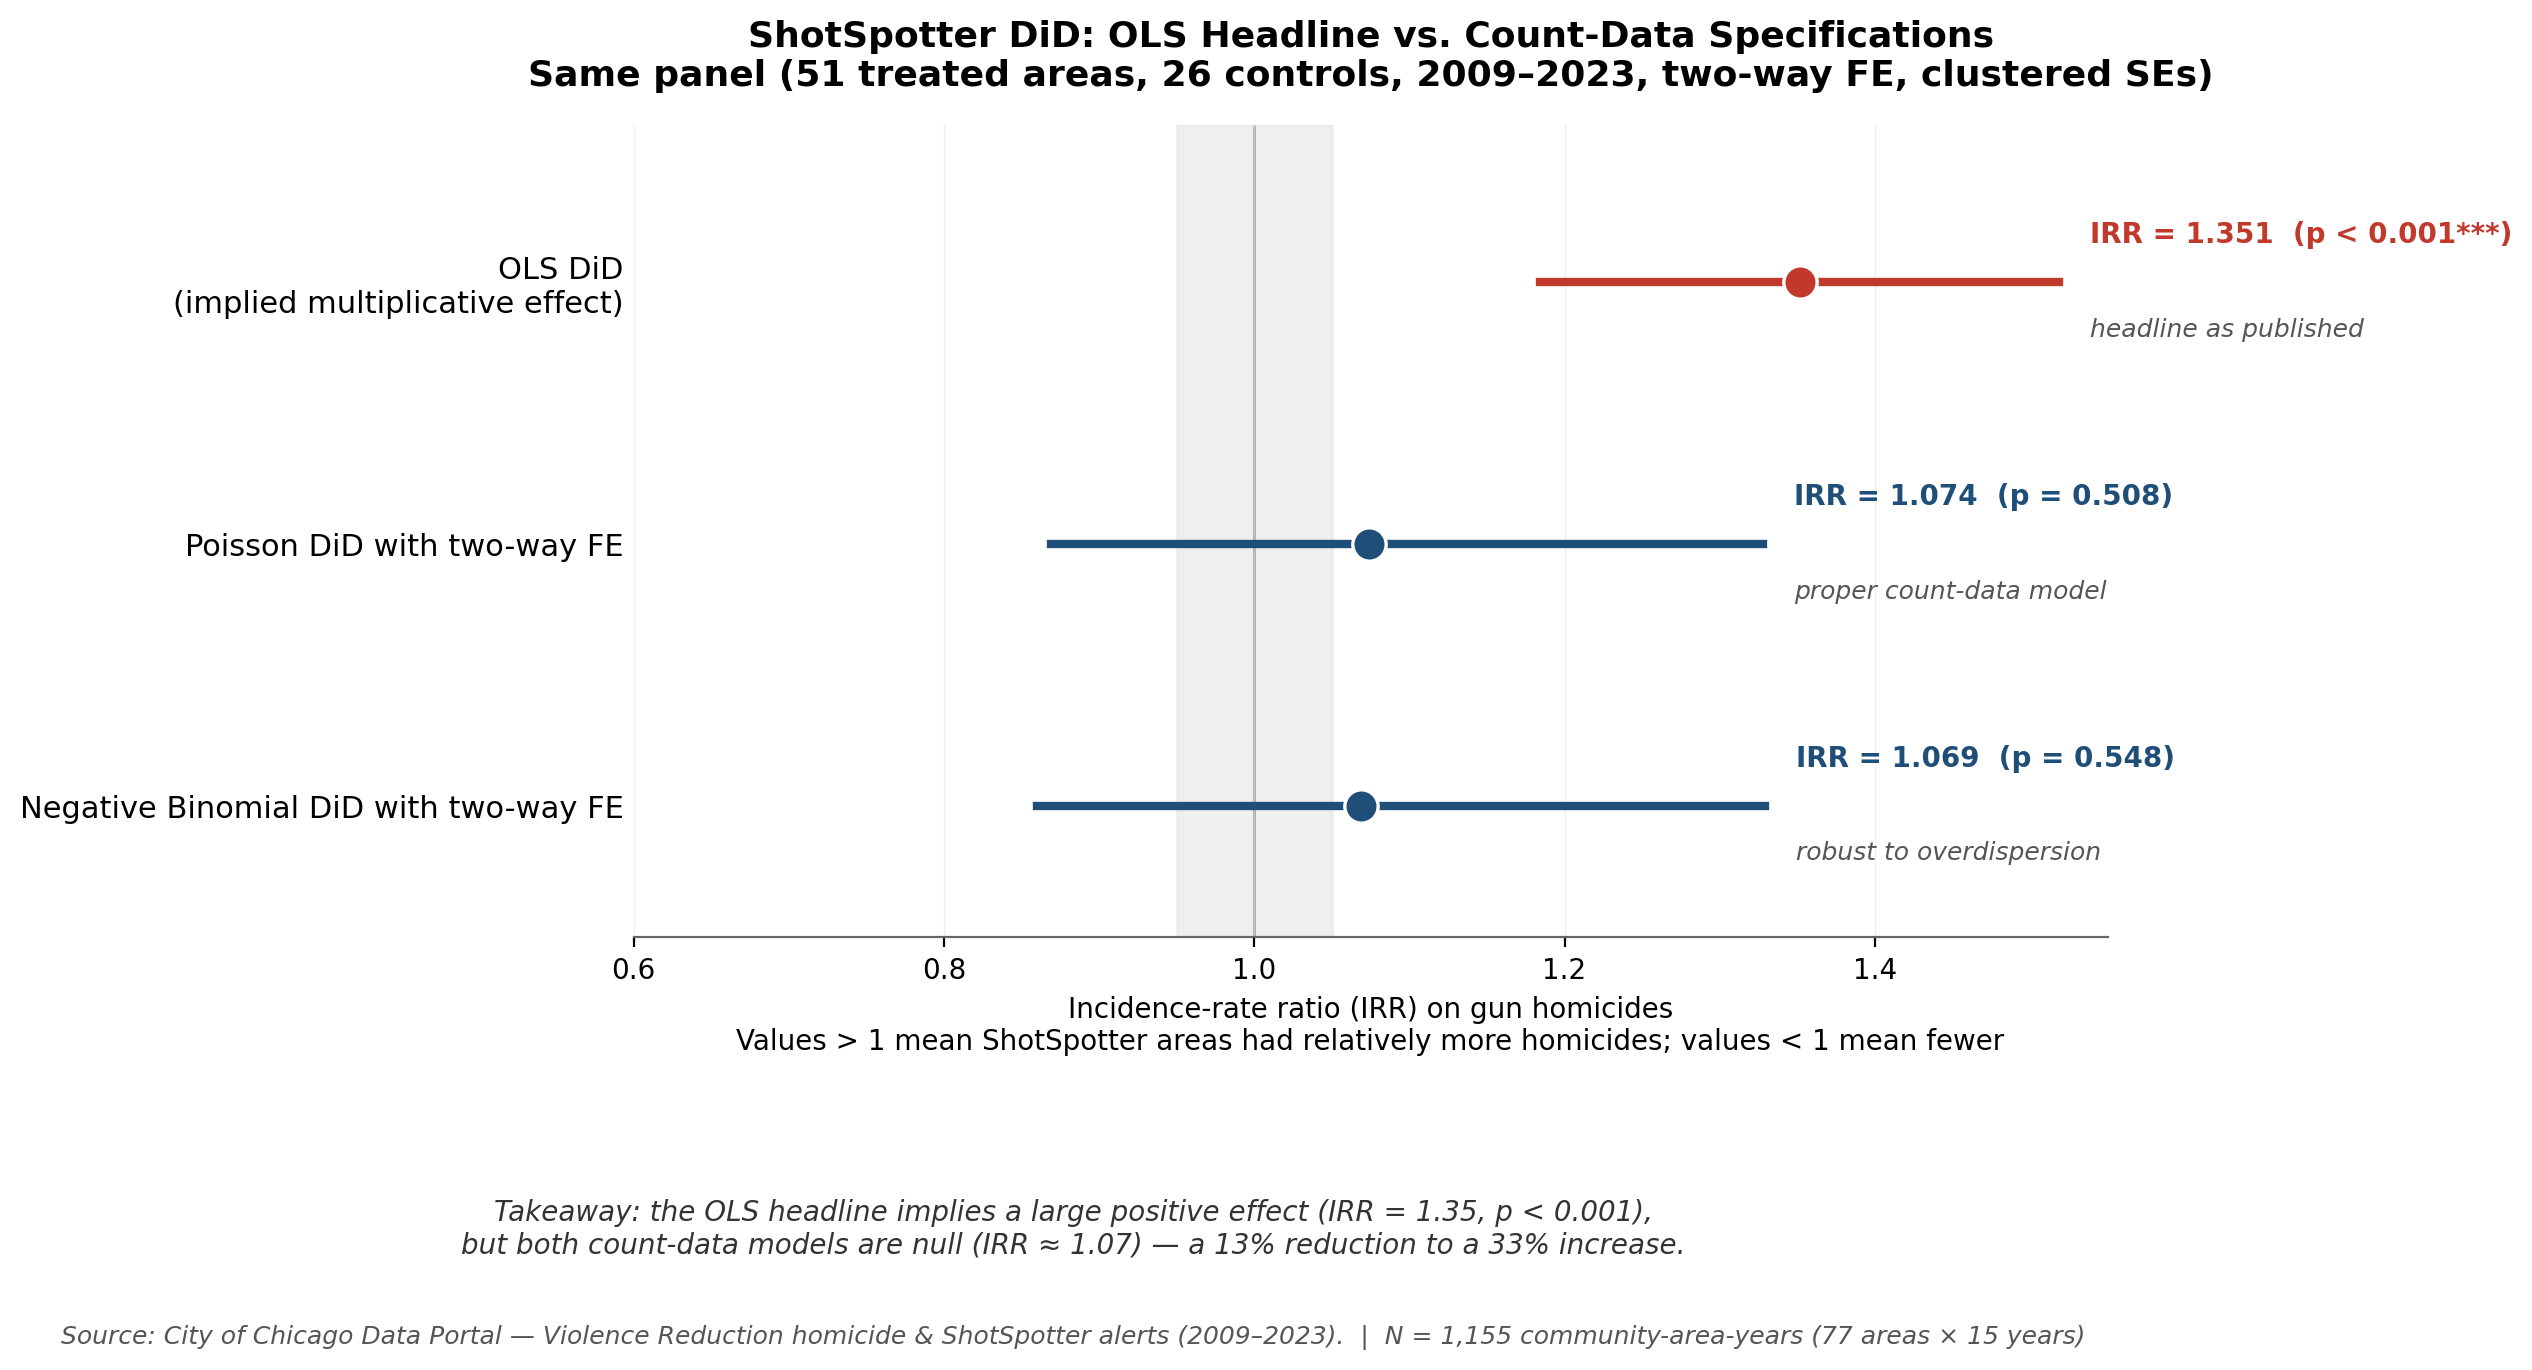
\includegraphics[width=0.82\textwidth]{specification_comparison.png}
\caption{Treatment effect by estimator. The ordinary least squares coefficient appears on
the multiplicative scale for comparison (implied incidence-rate ratio $1.35$, $p <
0.001$). The Poisson and Negative Binomial points are estimated incidence-rate ratios,
both statistically null near $1.07$.}
\label{fig:spec}
\end{figure}

\subsection{The design fails falsification}

If the post-2017 estimate measured a treatment effect, the same regression with treatment
assigned to years before ShotSpotter existed should return nothing. It does not. Placebo
treatment in 1999 yields $-1.34$ ($p = 0.008$) and in 2003 yields $-1.93$ ($p = 0.007$),
both significant at the 1\% level and comparable in magnitude to the post-2017 estimate
(Table~\ref{tab:placebo}). The placebo coefficients are negative while the real estimate
is positive. The opposite sign does not rescue the design; it shows that the specification
detects pre-existing differences in neighborhood trajectories, which appear whatever year
is labeled as treatment.

The stronger evidence is direction-free. A joint Wald test on the seven pre-treatment
interaction coefficients of the event study rejects parallel trends ($F = 19.9$, $p =
0.006$). The cohort-aware event study makes the violation visible
(Figure~\ref{fig:event}): every pre-treatment coefficient is large and negative, an
artifact of 2016, a record homicide year concentrated in the soon-to-be-treated areas,
sitting next to the base period. Once a design fails this test, the post-treatment
contrast cannot be read as causal.

\begin{table}[H]
\centering
\small
\caption{Placebo tests. Treatment is reassigned to years before the ShotSpotter rollout.}
\label{tab:placebo}
\begin{tabular}{lcccc}
\toprule
Fake treatment year & $\beta$ & SE & $p$ & 95\% CI \\
\midrule
1999 & $-1.344$ & 0.507 & 0.008 & $[-2.34, -0.35]$ \\
2003 & $-1.929$ & 0.714 & 0.007 & $[-3.33, -0.53]$ \\
2007 & $-0.645$ & 0.497 & 0.194 & $[-1.62, +0.33]$ \\
2011 & $+0.256$ & 0.347 & 0.461 & $[-0.42, +0.94]$ \\
\bottomrule
\end{tabular}
\end{table}

\begin{figure}[H]
\centering
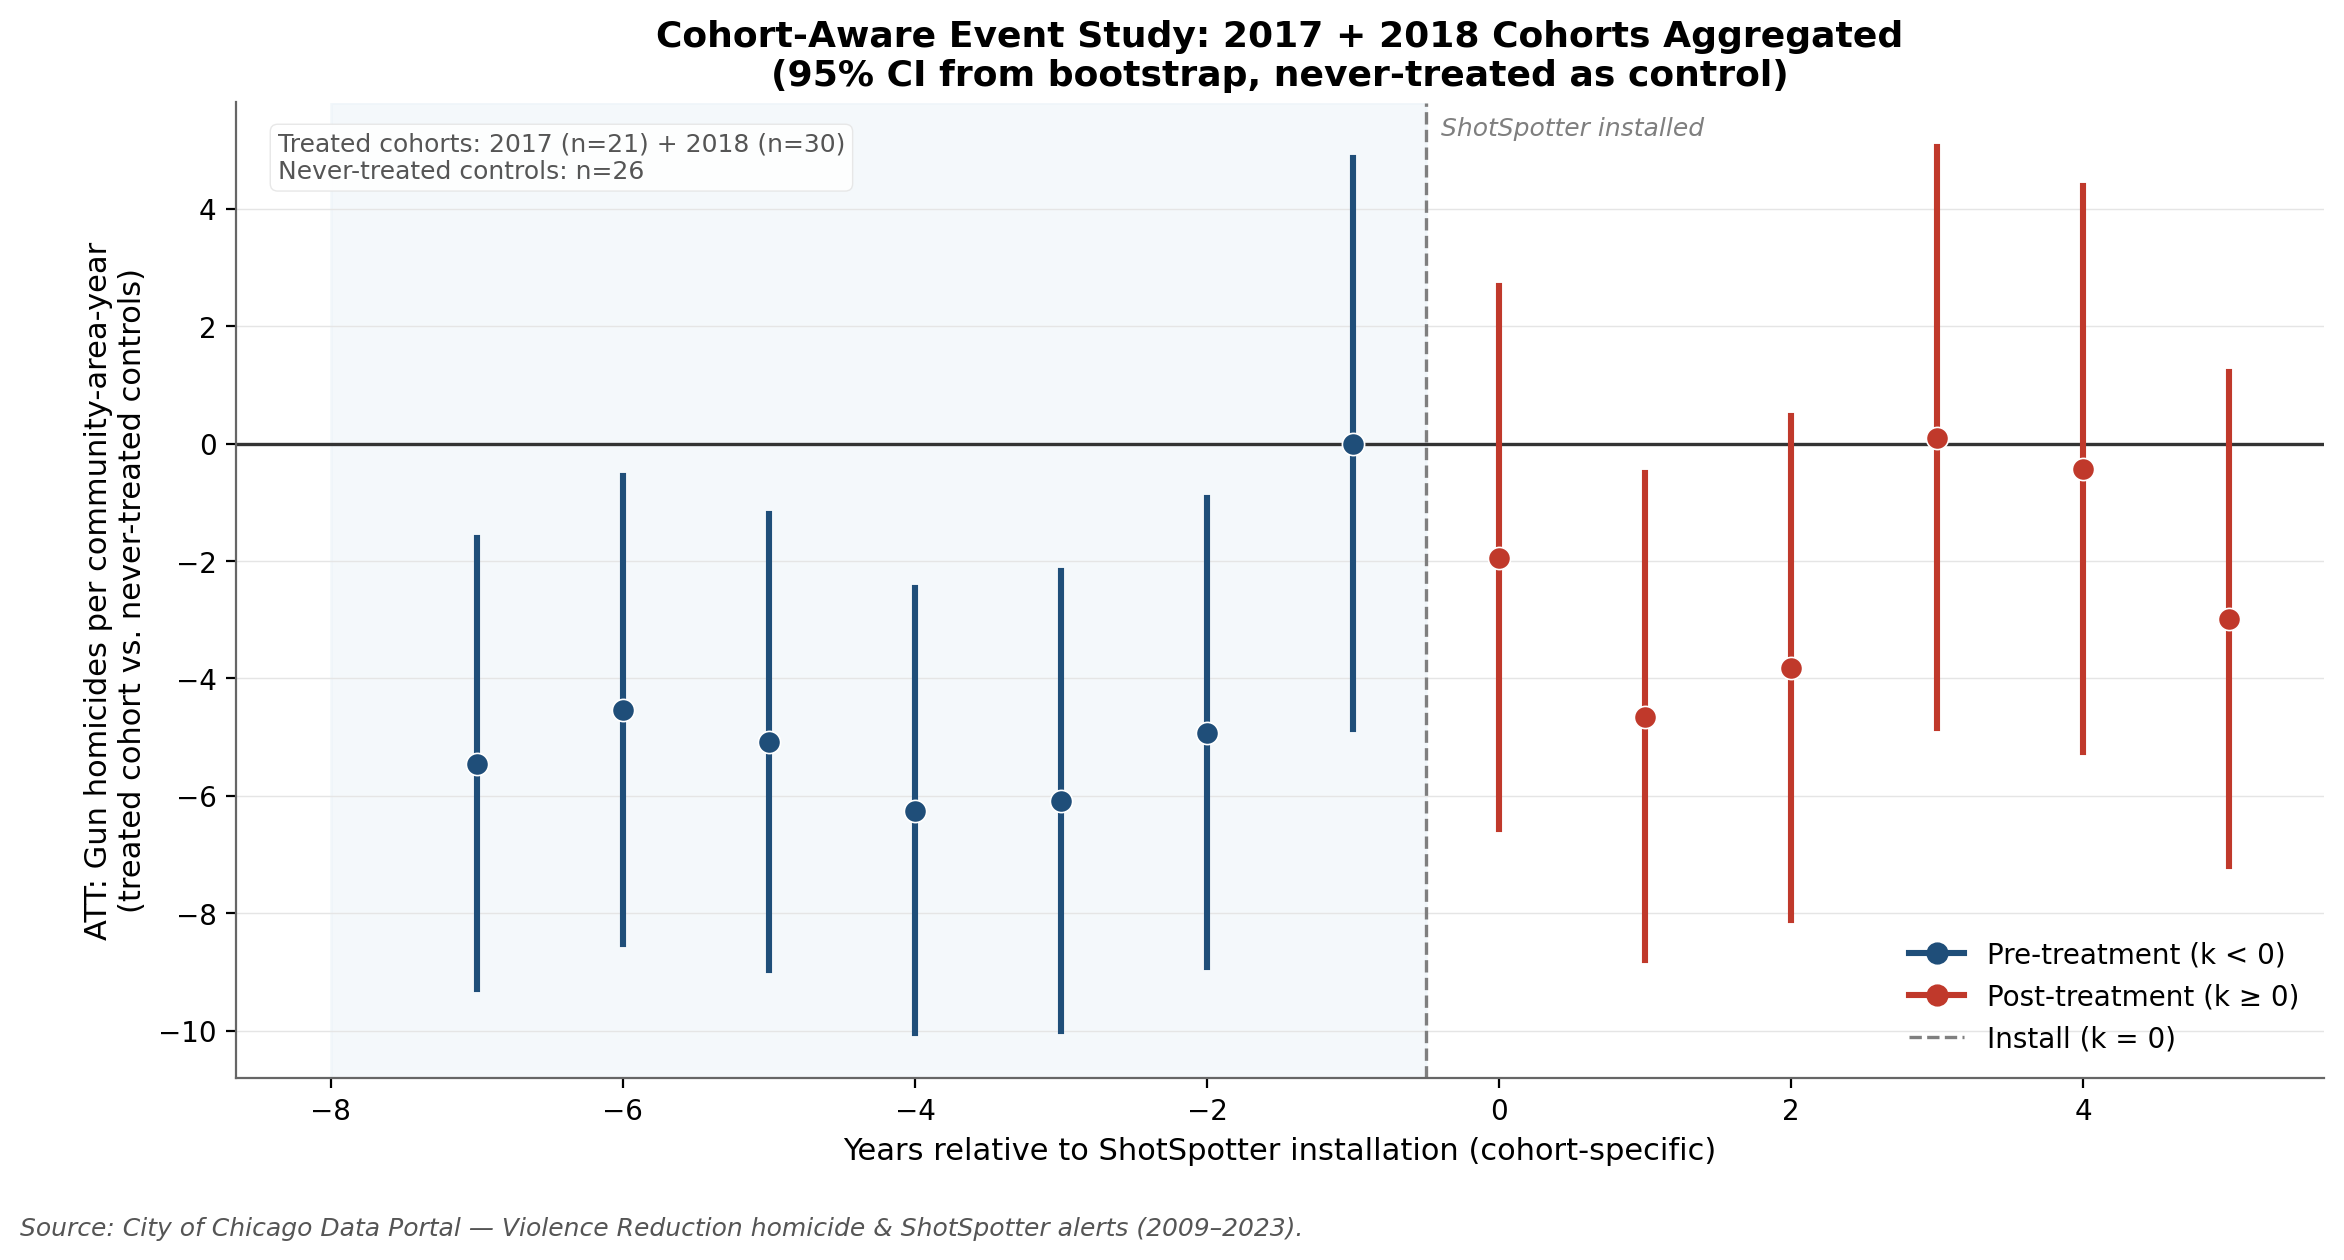
\includegraphics[width=0.82\textwidth]{event_study_cohort_aware.png}
\caption{Cohort-aware event study with bootstrap confidence intervals. Large negative
pre-treatment coefficients indicate a parallel-trends violation driven by the 2016 record
homicide year adjacent to the base period.}
\label{fig:event}
\end{figure}

\subsection{No valid comparison group}

A synthetic control (Abadie, Diamond, \& Hainmueller, 2010) would build a counterfactual
for each treated neighborhood from a weighted average of untreated areas. Here the
construction fails. For all six study neighborhoods the optimizer places 100\% of the
weight on a single donor, Washington Heights, the most violent never-treated area, and the
pre-treatment root mean squared error is 10 to 34 homicides per year against outcome
levels of 15 to 70. The synthetic series sits well below the actual series even within the
pre-treatment window it was fit to (Figure~\ref{fig:synth}). Permutation inference returns
a $p$-value below $0.001$ for every treated unit, but that rejection follows from the
level mismatch, not from a treatment effect. The never-treated areas occupy the
low-violence end of the city, so no weighted combination reproduces a high-violence
treated unit. The infeasibility is a property of the data: the city installed ShotSpotter
in every high-violence neighborhood and left no comparable unit untreated.

\begin{figure}[H]
\centering
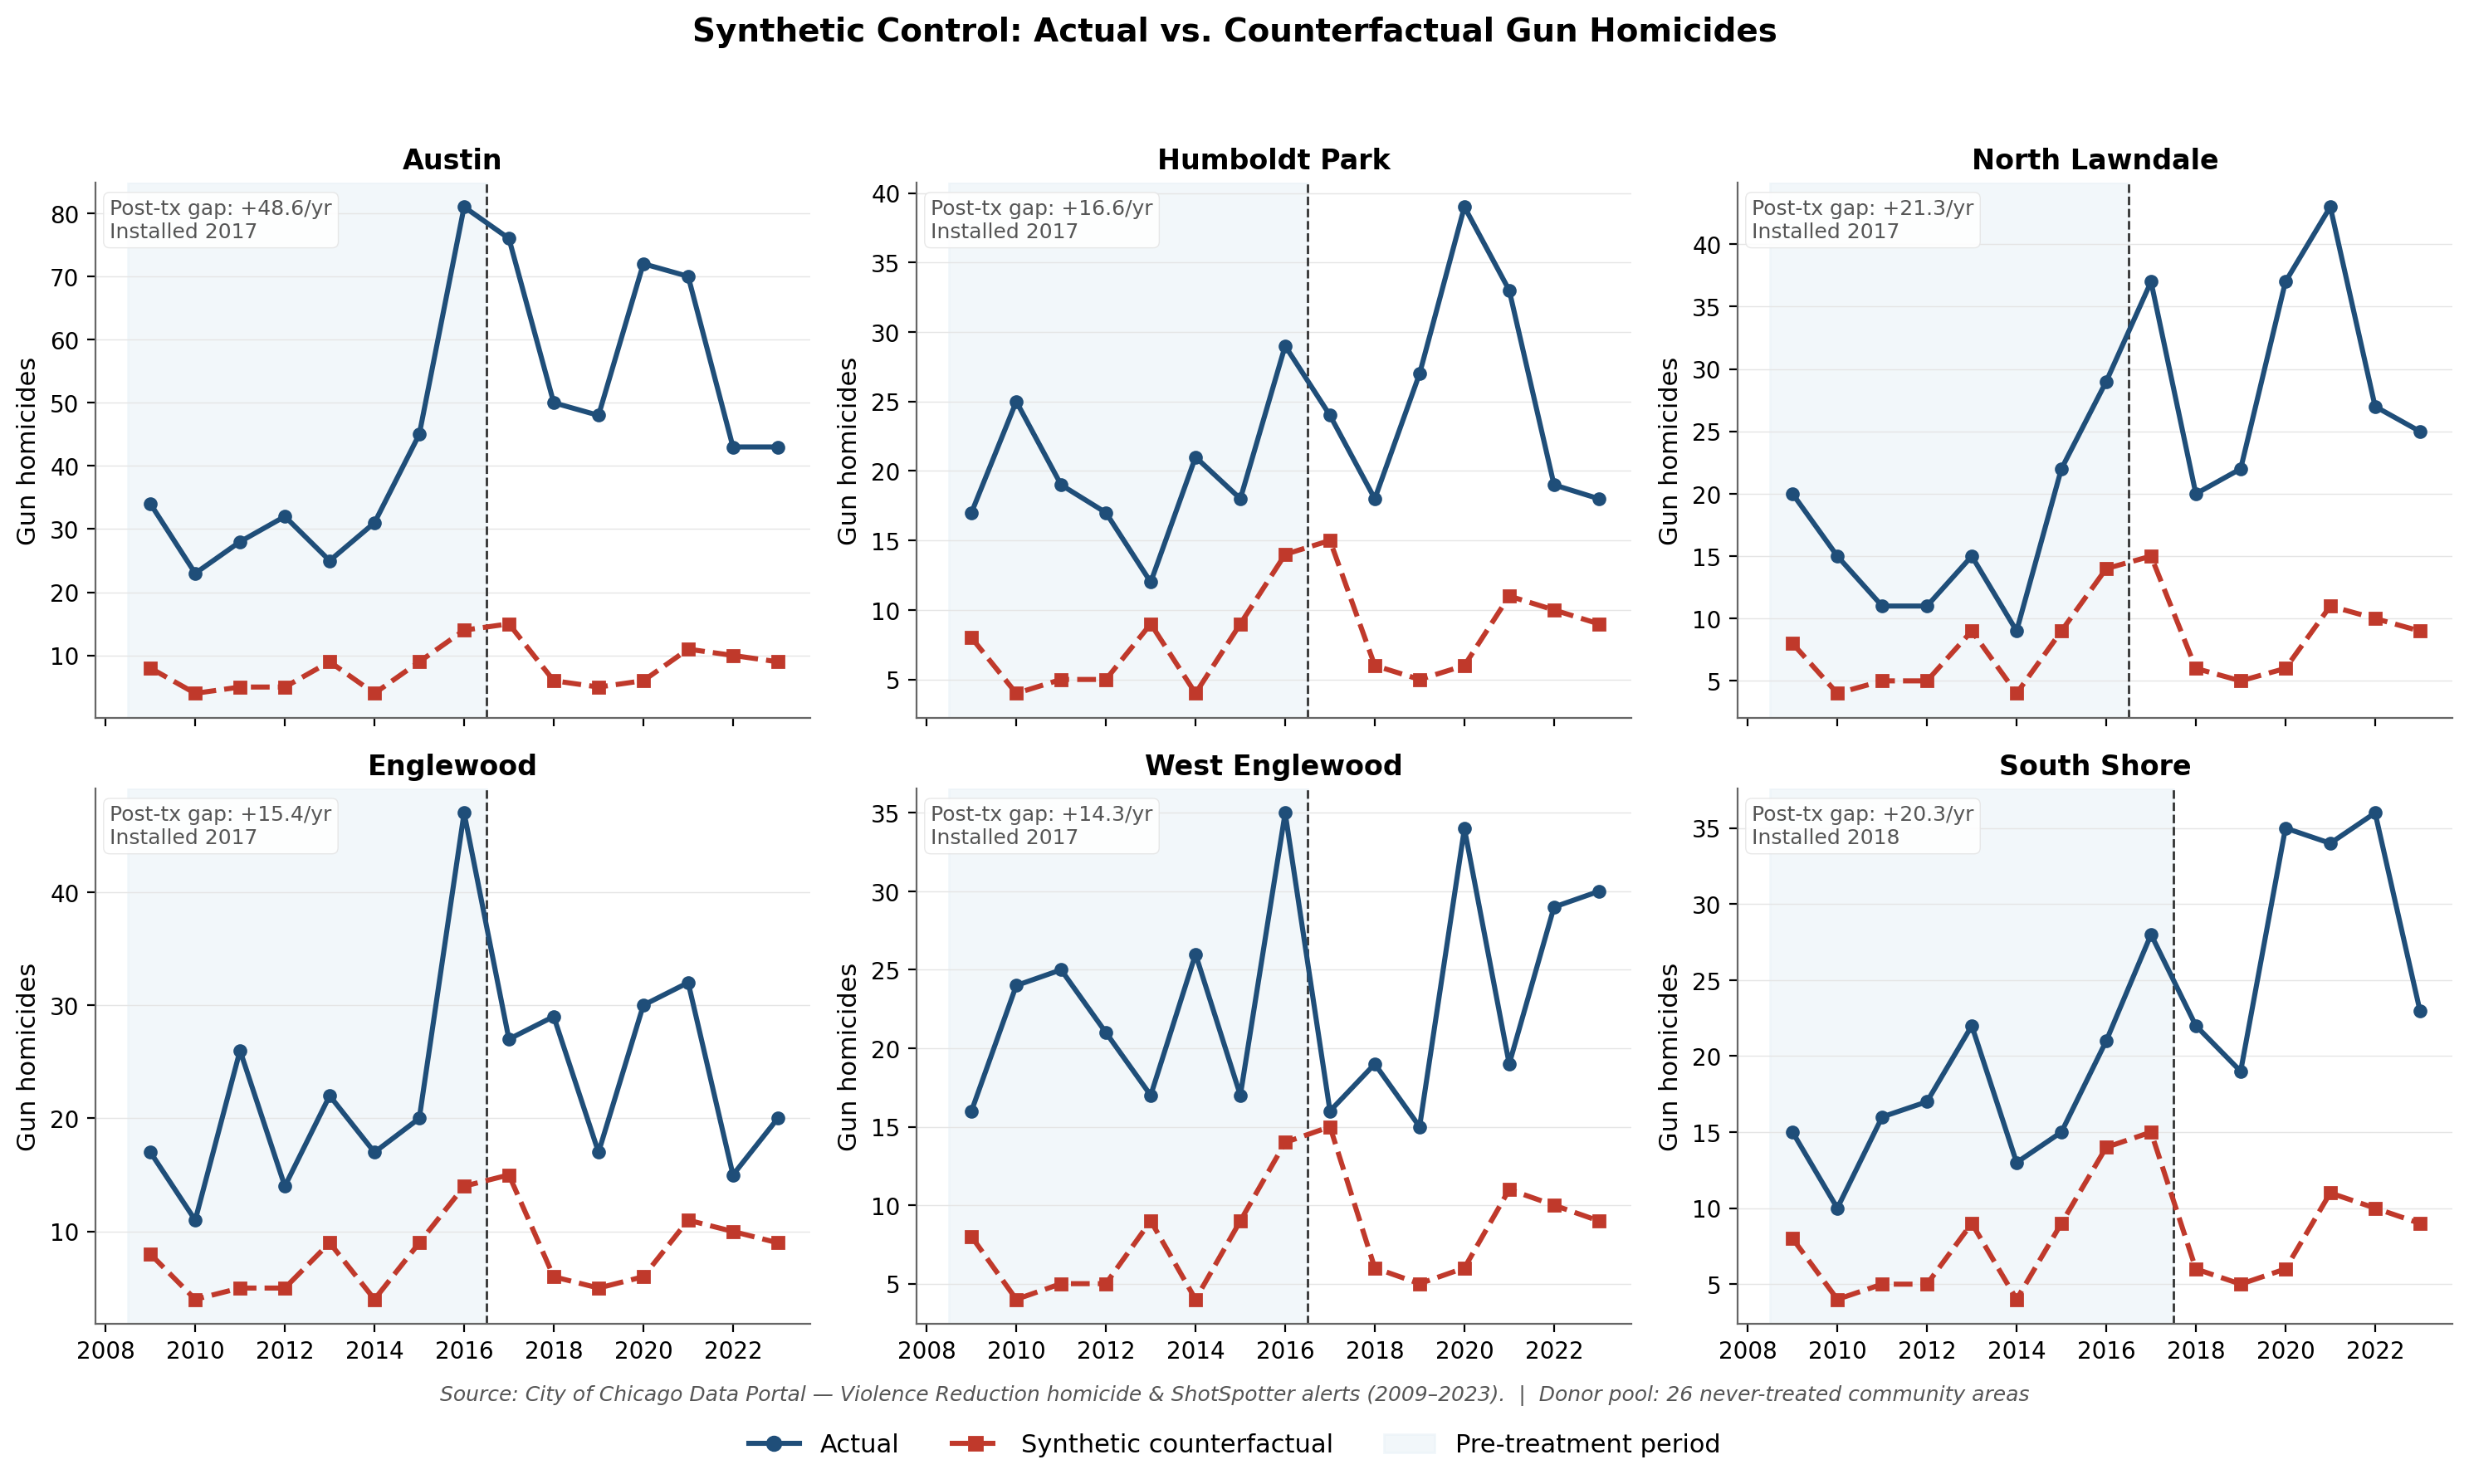
\includegraphics[width=\textwidth]{synthetic_control_panels.png}
\caption{Synthetic control for the six study neighborhoods. The synthetic series (red)
lies below the actual series (blue) even in the pre-treatment window it was fit to, because
no combination of lower-violence never-treated areas matches a high-violence treated unit.}
\label{fig:synth}
\end{figure}

\subsection{The modern estimator does not restore identification}

The Callaway and Sant'Anna (2021) estimator handles staggered adoption without the
negative weighting that biases two-way fixed effects under treatment-timing variation. On
the full panel its overall effect is $-2.45$ per area-year (SE $0.89$), negative and
opposite in sign to the pooled regression, and stable to using not-yet-treated controls
($-2.51$, Table~\ref{tab:cs}). The sign is not a property of the estimator. It rests on
the single 2016 pre-coefficient; the event study shows only that coefficient is
significant while the rest sit near zero, and dropping 2016 returns $+1.90$ (SE $0.72$),
the sign of the pooled regression. Three estimators give three answers: $+2.63$ from
ordinary least squares, a null ratio of $1.07$ from the count models, and $-2.45$
reversing to $+1.90$ from Callaway and Sant'Anna. The spread is not estimator disagreement
about a fixed parameter. It indicates a parameter the data do not pin down.

\begin{table}[H]
\centering
\small
\caption{Callaway and Sant'Anna (2021) overall effect, gun homicides per
community-area-year.}
\label{tab:cs}
\begin{tabular}{lcc}
\toprule
Control group & Overall effect & SE \\
\midrule
Never-treated                 & $-2.453$ & 0.893 \\
Not-yet-treated               & $-2.508$ & 0.898 \\
Never-treated, excl.\ 2016    & $+1.895$ & 0.724 \\
\bottomrule
\end{tabular}
\end{table}

\section{What the data support}

The results bound the answer without identifying it. The data do not show that ShotSpotter
increased gun homicides, because the $+2.63$ estimate is a scale artifact. They do not show
a reduction, because reading the negative event-study coefficients literally ignores that
the base year is anomalous. The count-data confidence interval spans a 13\% reduction to a
33\% increase, the full policy-relevant range.

One conclusion survives. The data are inconsistent with a large \emph{deterrence} effect.
An intervention large enough to justify a \$3 million detection contract would leave
negative post-treatment coefficients with intervals excluding zero, stability across
specifications, and a clearer signal in the higher-powered non-fatal-shooting series,
which carries about 30,000 events. None of these appears. These data bound only the
deterrence channel, however: a survival-channel mortality benefit of the size a boundary
regression discontinuity attributes to faster emergency response (University of Chicago
Crime Lab, 2024; not peer-reviewed) lies inside the count-model confidence interval and
would be invisible in an area-by-year homicide panel. Whatever effect ShotSpotter had on
homicides through deterrence was too small to separate from noise, from the 2016 anomaly,
and from pre-existing trend differences across neighborhoods.

\section{A better-identified design}

A credible evaluation needs a counterfactual these data do not contain. Three designs
would supply one. A geographic regression discontinuity at coverage boundaries would
compare blocks just inside and just outside a ShotSpotter zone, holding neighborhood
conditions roughly constant; it requires the sensor-coverage polygons, which the city has
not released. Estimation at finer resolution, census tract by month rather than community
area by year, would recover the within-neighborhood timing variation that the annual panel
averages away. Direct measurement of the mechanism, police response time and time to
trauma care around each activation date, would test the channel through which detection
could reduce deaths instead of inferring it from counts. Each design targets the failure
documented above, the absence of a comparable untreated unit.

\section{Conclusion}

ShotSpotter detected gunfire. Alert volume rose in covered areas because the sensors
measure shots that 911 calls miss. The evaluation question is different, and these data
answer it only in the negative. A significant difference-in-differences coefficient
dissolves under a count model, a parallel-trends test, and a pre-rollout placebo, the
comparison group cannot be constructed, and the modern staggered-adoption estimator
changes sign on one year. With no clean counterfactual and a pre-period dominated by an
outlier, the data cannot identify the effect of ShotSpotter on gun homicides in either
direction. The 2023 decision to end the contract is consistent with that absence of
evidence. The wider lesson carries to any program evaluated this way: a coefficient that
survives fixed effects and robustness restrictions can still fail the conditions a causal
reading requires.

\section*{References}
\begin{flushleft}
\setlength{\parindent}{-0.4in}
\leftskip=0.4in

Abadie, A., Diamond, A., \& Hainmueller, J. (2010). Synthetic control methods for
comparative case studies: Estimating the effect of California's tobacco control program.
\emph{Journal of the American Statistical Association, 105}(490), 493--505.

Callaway, B., \& Sant'Anna, P. H. C. (2021). Difference-in-differences with multiple time
periods. \emph{Journal of Econometrics, 225}(2), 200--230.

Cameron, A. C., \& Trivedi, P. K. (2013). \emph{Regression analysis of count data} (2nd
ed.). Cambridge University Press.

Choi, K. S., Librett, M., \& Collins, T. J. (2014). An empirical evaluation: Gunshot
detection system and its effectiveness on police practices. \emph{Police Practice and
Research, 15}(1), 48--61.

Connealy, N. T., Piza, E. L., Arietti, R. A., Carter, J. G., \& Mohler, G. (2024).
Staggered deployment of gunshot detection technology in Chicago, IL: A matched
quasi-experiment of gun violence outcomes. \emph{Journal of Experimental Criminology,
20}(4), 1027--1053.

Doucette, M. L., Green, C., Necci Dineen, J., Shapiro, D., \& Raissian, K. M. (2021).
Impact of ShotSpotter technology on firearm homicides and arrests among large
metropolitan counties: A longitudinal analysis, 1999--2016. \emph{Journal of Urban
Health, 98}(5), 609--621.

Goodman-Bacon, A. (2021). Difference-in-differences with variation in treatment timing.
\emph{Journal of Econometrics, 225}(2), 254--277.

Irvin-Erickson, Y., Bai, B., Gurvis, A., \& Mohr, E. (2016). \emph{The effect of gun
violence on local economies}. Urban Institute.

Office of Inspector General, City of Chicago. (2021, August 24). \emph{The Chicago Police
Department's use of ShotSpotter technology}.

University of Chicago Crime Lab. (2024). Op-ed and replication analysis of ShotSpotter and
shooting fatality in Chicago [not peer-reviewed].

\end{flushleft}

\end{document}
